\documentclass[12pt]{article}
\usepackage{amsmath}
\usepackage{array}
% \usepackage{gensymb}
\usepackage{geometry}
\usepackage{graphicx}
\usepackage{pgfplots}
\usepackage{siunitx}
\usepackage{wrapfig}

\title{Homework \#16}
\author{Donald Aingworth IV}
\date{December 11, 2024}

\pgfplotsset{width=8cm,compat=1.9}
\usepgfplotslibrary{external}
% \tikzexternalize

\begin{document}

\DeclareSIUnit{\mile}{mi}
\DeclareSIUnit{\gal}{gal}
\DeclareSIUnit{\foot}{ft}
\DeclareSIUnit{\hour}{h}
\DeclareSIUnit{\rad}{rad}
\DeclareSIUnit{\unit}{u}
\DeclareSIUnit{\dyne}{dyn}

\maketitle

\pagebreak
\section*{Question 2}
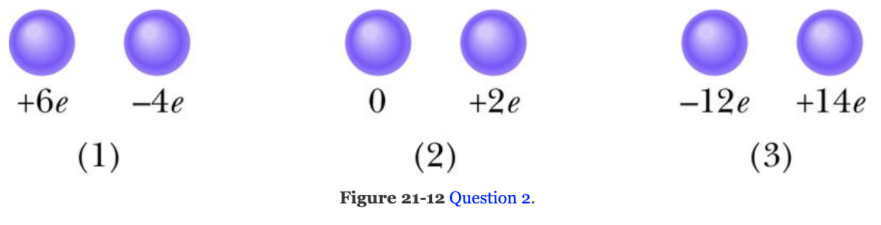
\includegraphics[width=\textwidth]{picture_1.png}
Figure 21-12 shows three pairs of identical spheres that are to be touched together and then separated. The initial charges on them are indicated. Rank the pairs according to (a) the magnitude of the charge transferred during touching and (b) the charge left on the positively charged sphere, greatest first.

\subsection*{Solution}
a) (3) $>$ (1) $>$ (2)\\
In this problem, we just need to rank the differences between the charges on the balls. In instance 1, the difference is $6 - (-4) = 10$. In instance 2, the difference is $2 - 0 = 2$. In instance 3, the difference is $14 - (-12) = 26$. We can then rank the three, and the result is \boxed{(3) > (1) > (2)}.\\
b) (1) = (2) = (3)
In this In this problem, we just need to rank the average charge of each of the two balls. In instance 1, the average is $\frac{6 + (-4)}{2} = 1$. In instance 2, the difference is $\frac{2 + 0}{2} = 1$. In instance 3, the difference is $\frac{14 + (-12)}{2} = 1$. We can then rank the three, and the result is \boxed{(1) = (2) = (3)}.


\pagebreak
\section*{Question 8}
% \begin{wrapfigure}{r}{0.15\textwidth}
%     \vspace{-30pt}
    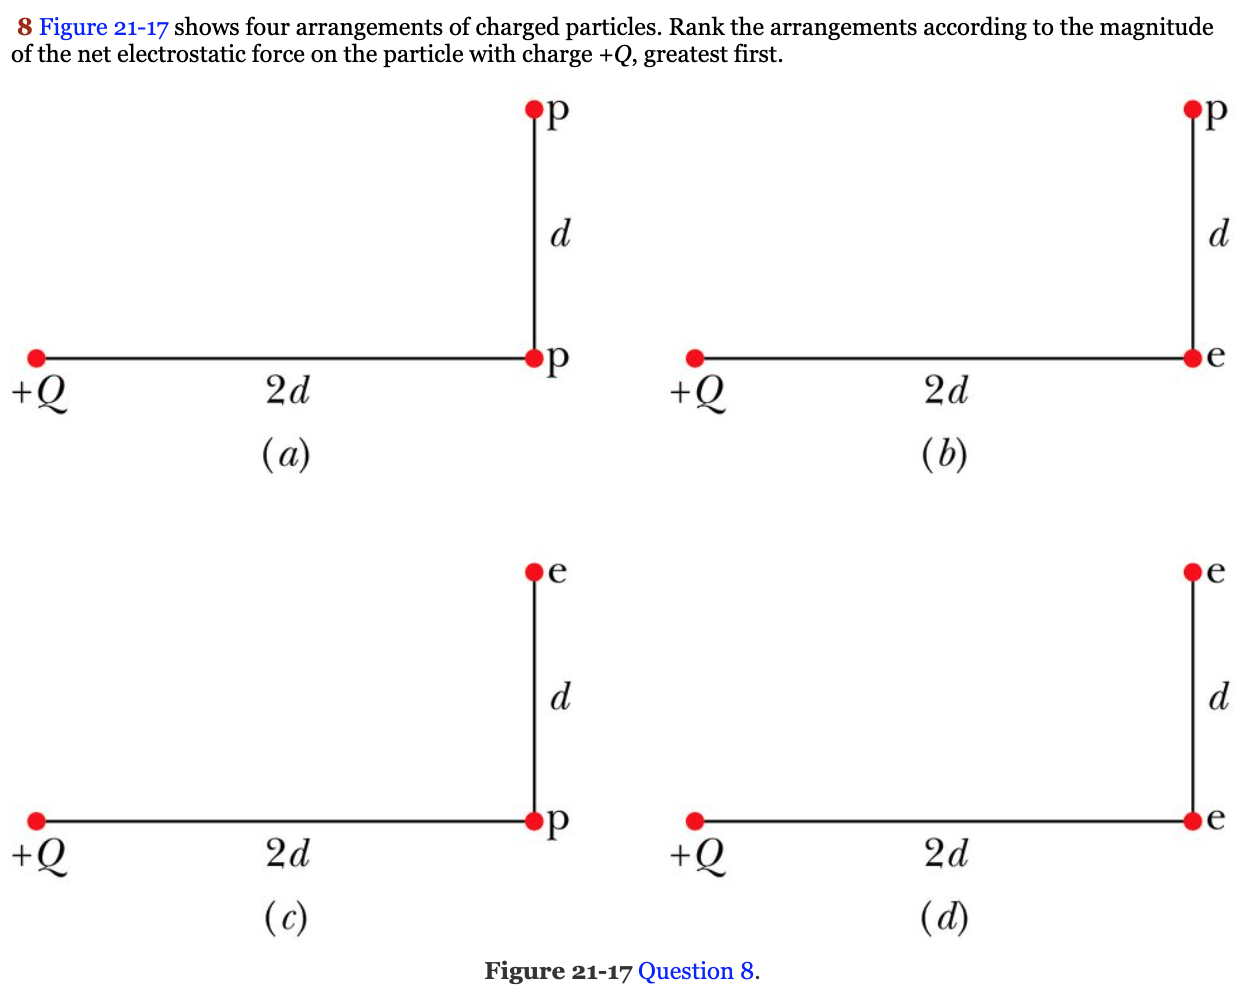
\includegraphics[width=\textwidth]{picture_2.png} 
%     % \label{fig:wrapfig}
% \end{wrapfigure}

\subsection*{Solution}



\pagebreak
\section*{Question 10}
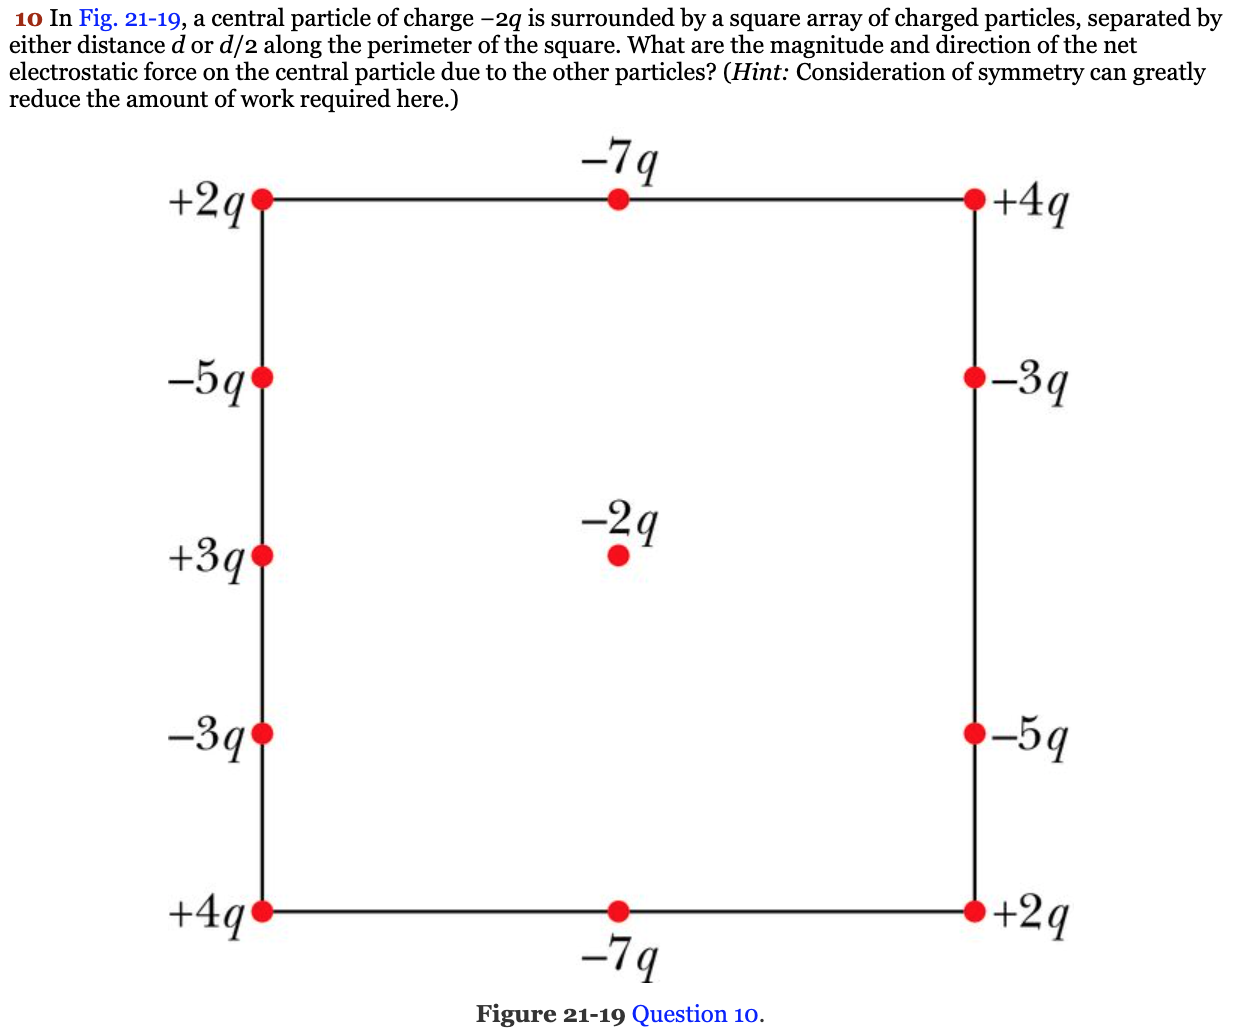
\includegraphics[width=\textwidth]{picture_3.png} 

\pagebreak
\section*{Problem 10}
\begin{wrapfigure}{r}{0.25\textwidth}
    \vspace{-50pt}
    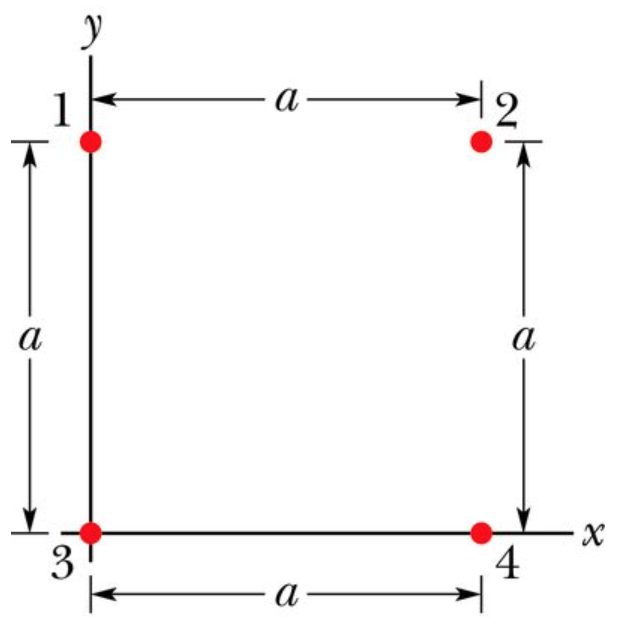
\includegraphics[width=0.25\textwidth,height=0.25\textwidth]{picture_4.png} 
    % \label{fig:wrapfig}
\end{wrapfigure}
In Fig. 21-25, four particles form a square. The charges are $q_1 = q_4 = Q$ and $q_2 = q_3 = q$. (a) What is Q/q if the net electrostatic force on particles 1 and 4 is zero? (b) Is there any value of q that makes the net electrostatic force on each of the four particles zero? Explain.

\subsection*{Solution}
The distance between particles 1 and 4 is found by the pythagorean theorem.
\[r_{14} = r_{23} = \sqrt{a^2 + a^2} = a\sqrt{2}\]

\subsubsection*{(a) Find Q/q}
From this, we know that net electrostatic force on 1 from 4 in the direction of the line between 1 and 2 has to be equal to the force on 1 from 4. Roughly the same applies in the direction of the line between 1 and 3. As such, we can write a formula for the net force (which is 0).
\begin{align*}
    F_{net} = 0 = \frac{k\left|q_1\right|\left|q_2\right|}{r^2} &- \frac{k\left|q_1\right|\left|q_4\right|}{r^2}*\cos(\theta)\\
    \frac{k\left|q_1\right|\left|q_2\right|}{r^2} &= \frac{k\left|q_1\right|\left|q_4\right|}{r^2}*\cos(\theta)\\
    \frac{\left|q_2\right|}{a^2} &= \frac{\left|q_4\right|}{2a^2}*\frac{\sqrt{2}}{2}\\
    \frac{\left|q_4\right|}{\left|q_2\right|} &= \frac{4}{\sqrt{2}} = 2\sqrt{2}
\end{align*}
Since the forces must be in opposite directions, the charges must be opposite, so the ration has to be negative. This means that \boxed{Q/q = -2\sqrt{2}}.

\subsubsection*{(b)}


\pagebreak
\section*{Problem 11}
% \begin{wrapfigure}{r}{0.25\textwidth}
%     \vspace{-30pt}
%     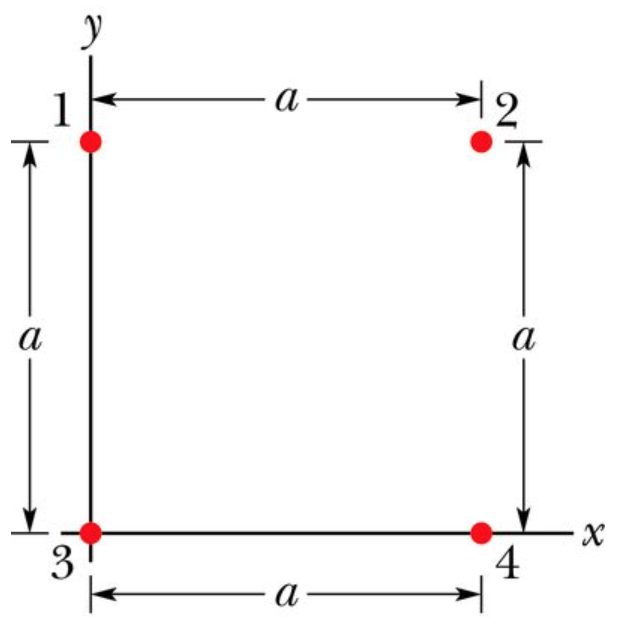
\includegraphics[width=0.25\textwidth]{picture_4.png} 
%     % \label{fig:wrapfig}
% \end{wrapfigure}
In Fig. 21-25, the particles have charges $q_1 = -q_2 = 100 \unit{\nano\coulomb}$ and $q_3 = -q_4 = 200 \unit{\nano\coulomb}$, and distance $a = 5.0\unit{\centi\meter}$. What are the (a) x and (b) y components of the net electrostatic force on particle 3?

\subsection*{Solution}



\pagebreak
\section*{Problem 23}
\begin{wrapfigure}{r}{0.25\textwidth}
    \vspace{-30pt}
    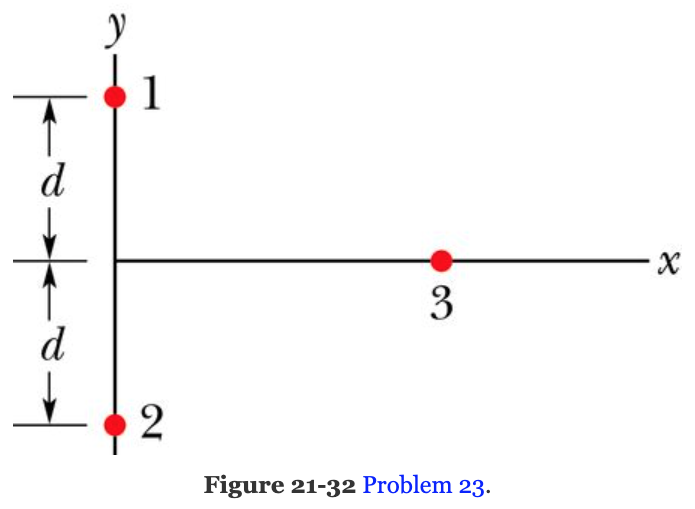
\includegraphics[width=0.25\textwidth]{picture_6.png} 
    % \label{fig:wrapfig}
\end{wrapfigure}
Fig. 21-32, particles 1 and 2 of charge 91 = Q2 = +3.20 × 10-19 C are on a y axis at distance d = 17.0 cm from the origin. Particle 3 of charge 93 = +6.40 × 10-19 C is moved gradually along the x axis from x = O to x = +5.0 m. At what values of x will the magnitude of the electrostatic force on the third particle from the other two particles be (a) minimum and (b) maximum? What are the (c) minimum and (d) maximum magnitudes?

\pagebreak
\section*{Problem 31}
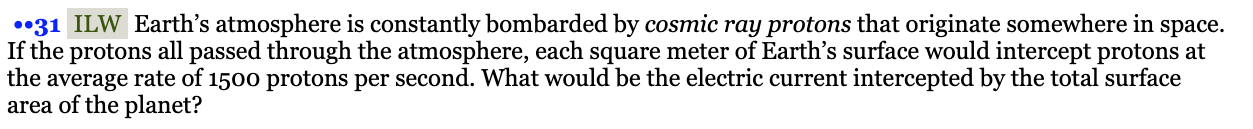
\includegraphics[width=\textwidth]{picture_7.png} 

\pagebreak
\section*{Problem 36}
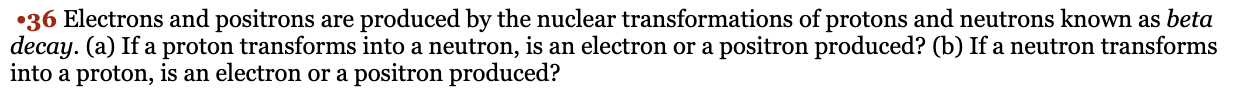
\includegraphics[width=\textwidth]{picture_8.png} 


\end{document}